% "{'classe':('PSI'),'chapitre':'slci_rapidite','type':('td'),'titre':'Base TC200 Tecdron', 'source':'Centrale Supelec TSI 2021','comp':['C2-03',],'corrige':False}"
%\setchapterimage{fig_00_bis}
\chapter*{TD \arabic{cptTD} \\ 
Base TC200 Tecdron -- \ifprof Corrigé \else Sujet \fi}

\addcontentsline{toc}{section}{TD \arabic{cptTD} : Base TC200 Tecdron -- \ifprof Corrigé \else Sujet \fi}

\iflivret \stepcounter{cptTD} \else
\ifprof  \stepcounter{cptTD} \else \fi
\fi
\setcounter{question}{0}

\marginnote{Centrale Supelec TSI 2021.}
\marginnote{\UPSTIcompetence[2]{C2-03}}
\begin{marginfigure}
\centering
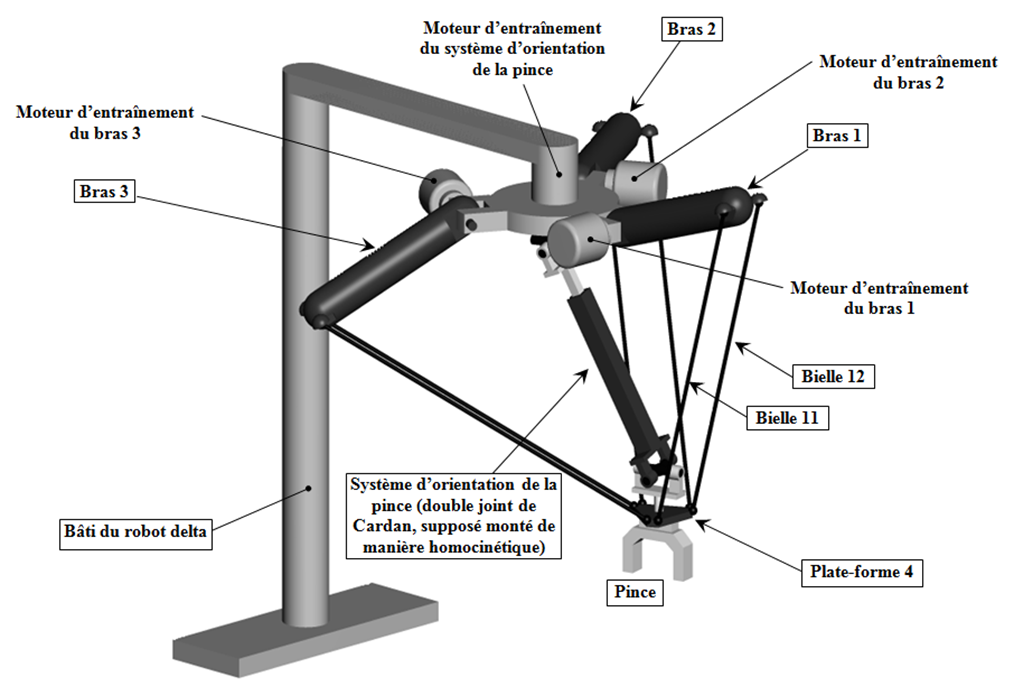
\includegraphics[width=\linewidth]{fig_01}
\end{marginfigure}



\subsection*{Mise en situation}

Dans l’industrie, il est désormais possible d’associer des tâches robotisées et des tâches manuelles. Après l’essor
des robots collaboratifs, Tecdron, entreprise Française basée à La Rochelle, propose une base mobile nommée
TC200, capable de recevoir différents types de bras robotisés -- dont des bras collaboratifs -- mais aussi de
se déplacer de manière autonome dans un environnement industriel complexe composé de robots et d’humains.

Les figures ci-après donnent la structure du robot étudié. 

\begin{marginfigure}
\centering
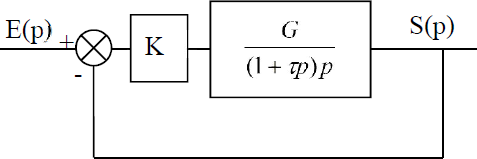
\includegraphics[width=\linewidth]{fig_02}

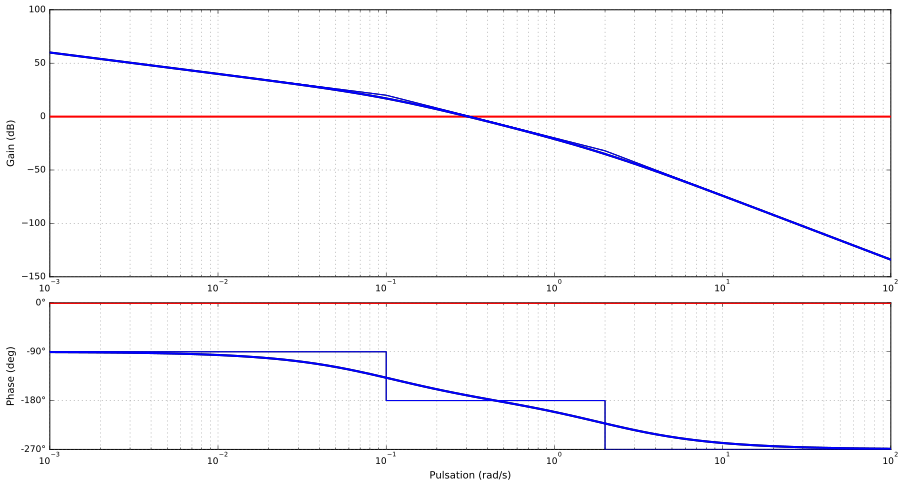
\includegraphics[width=\linewidth]{fig_03}
\end{marginfigure}




\subsection*{Validation de l'asservissement du moteur}
\begin{obj}
Valider l’asservissement de vitesse mis en place pour que la base TC200 se déplace suivant la trajectoire
de consigne souhaitée.

Vérifier les exigences de la boucle de vitesse en termes de stabilité, précision et rapidité.
\end{obj}


\footnotesize
\begin{table*}
\begin{tabular}{lp{11cm}p{4cm}}
\hline
\textbf{Exigence} & \textbf{Critère} & \textbf{Performance attendue} \\
\hline
\multirow{2}{*}{Précision} & 
Erreur relative en régime permanent $\mu_{v\infty}$ pour une consigne en échelon d'amplitude $\omega_{mc0}$ & $\mu_{v\infty} < \SI{1}{\%}$ \\
& Erreur en vitesse en régime permanent $\Delta \omega_{\infty}$ pour une consigne en rampe telle que $\omega_{mc}(t)  = at$ & $\leq \SI{100}{rad.s^{-1}}$ pour une pente de $\SI{1800}{rad.s^{-1}}$ \\
Rapidité & Temps de réponse à $\SI{5}{\%}$ & $\indice{t}{5\%} < \SI{180}{ms}$ \\
\multirow{2}{*}{Stabilité} & Dépassement maximal & $\leq \SI{10}{\%}$  \\
& Marge de phase & $\geq 60\degres$  \\
\hline
\end{tabular}
\end{table*}

\normalsize


La boucle de courant étant supposée parfaite, le schéma-blocs de la figure suivante correspond à l’asservissement de
vitesse d’une des motorisations. Le modèle est considéré pour le moment non perturbé, c’est-à-dire $C_f(p)=0$.

\begin{center}
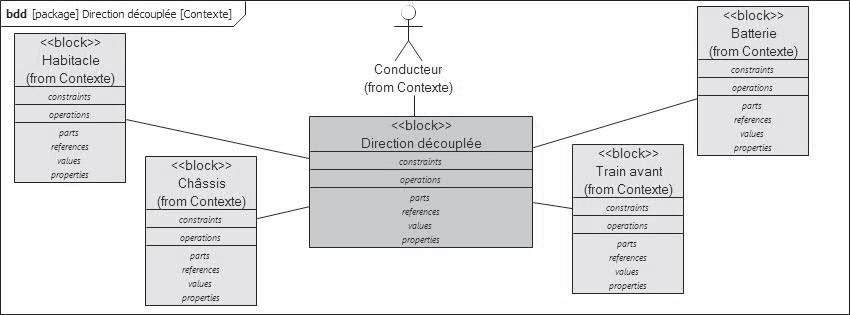
\includegraphics[width=\linewidth]{fig_05}
%\textit{}
\end{center}


\begin{center}
\begin{tabular}{lll}
\hline
\textbf{Fonction de transfert} & \textbf{Expression} & \textbf{Valeur} \\
\hline
Codeur et sa carte de traitement & $\indice{K}{cod}$ & $\SI{0,2}{V.s.rad^{-1}}$ \\
Constante de couple & $K_t$ & $\SI{0,09}{N.m.A^{-1}}$ \\
Correteur de type proportionnel & $C_2(p) = K_2 $ &  \\
Dynamique de la motorisation & $H_2(p)=\dfrac{1}{\indice{J}{eq}p}$ & $\indice{J}{eq} = 1,5\times 10^{-3} \si{kg.m^2}$ \\
\hline
\end{tabular}
\end{center}

\question{Déterminer la fonction de transfert en boucle fermée $\indice{H}{BF}(p)=\dfrac{\Omega_m(p)}{\Omega_{mc}(p)}$ pour $C_f(p)=0$.}
\ifprof
\begin{corrige}
\end{corrige}
\else
\fi

\question{Justifier que cet asservissement est stable et donner la valeur de la marge de phase.}
\ifprof
\begin{corrige}
\end{corrige}
\else
\fi


\question{Déterminer la condition sur $K_2$ afin de satisfaire l’exigence de rapidité.}
\ifprof
\begin{corrige}
\end{corrige}
\else
\fi


\question{Calculer l’erreur relative en régime permanent $\mu_{v \infty}$ pour une consigne de vitesse en échelon de valeur $\omega_{mc0}$.}
\ifprof
\begin{corrige}
\end{corrige}
\else
\fi

On donne les diagrammes de Bode de la FTBO.

\begin{center}
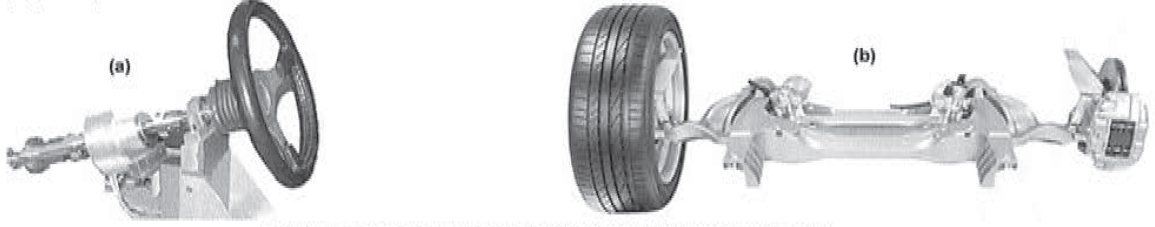
\includegraphics[width=\linewidth]{fig_07}
%\textit{}
\end{center}


\question{Identifier la valeur de $K_2$ qui a été réellement choisie par le constructeur.}
\ifprof
\begin{corrige}
\end{corrige}
\else
\fi

\question{À partir de cette valeur, calculer l’erreur en vitesse en régime permanent $\Delta \omega_{\infty}$ pour une consigne de vitesse en rampe de pente $a$ et valider le critère de précision des exigences.}
\ifprof
\begin{corrige}
\end{corrige}
\else
\fi

\ifprof
\else
\begin{marginfigure}[-3cm]
\centering

\includegraphics[width=3cm]{Cy_02_Ch_02_TD_03_qr}
\end{marginfigure}
\fi




%\subsection*{Éléments de correction}
%\begin{enumerate}
%\item ...
%\item $\left(Mp^2+\mu p + k \right)\Delta Z(p) = S\Delta p (p)-\Delta F(p)$ et $\Delta Q(p)=S p \Delta Z(p) + \left( \varphi + \dfrac{V}{2b} p \right) \Delta P(p)$.
%\item ...
%\item $\Delta q = K\Delta U\sqrt{p_a - P_0} - \dfrac{KU_0}{2\sqrt{p_a - P_0}}\Delta p + \text{termes néglig.}$.
%\item ...
%\item ...
%\item $K_a = k_c$.
%\item $\text{FTBO}(p)=\dfrac{ABC(p)GE}{1+GDB+GE}$ et $\text{FTBF}(p)=\dfrac{\text{FTBO}(p)}{1+\text{FTBO}(p)}$.
%\item ...
%\item ...
%\item ...
%\item $\omega_0=\SI{83,6}{rad.s^{-1}}$ et $\xi=0,21$, $\omega_3 = \SI{0,75}{rad.s^{-1}}$.
%\item ...
%\item ...
%\end{enumerate}





